The results of closed-loop simulations with the Optiwise simulation model equipped with either the MMG original or the quadratic model are shown in \autoref{fig:sim_optiwise}. There was very good agreement for the zigzag20/20 tests and a little less agreement for the zigzag10/10 tests, where the MMG quadratic was the better of the two models. Up to four degrees of deviation was observed between the overshoot angles, as shown in \autoref{fig:overshoots_optiwise}.   
\begin{figure}[h]
     \centering
     \begin{subfigure}[b]{0.40\textwidth}
         \centering
         \includesvg{figures/results_optiwise_ID.closed loop zigzag 10_10 port.svg}
         %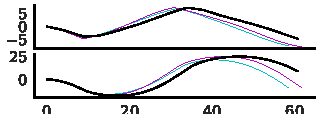
\includegraphics[]{figures/results_optiwise_ID.closed loop zigzag 10_10 port.pdf}
        \caption{Zigzag10/10 to port.}
        \label{fig:sim_optiwise_10_port}
     \end{subfigure}
     \hfill
     \begin{subfigure}[b]{0.40\textwidth}
         \includesvg{figures/results_optiwise_ID.closed loop zigzag 10_10 stbd.svg}
         %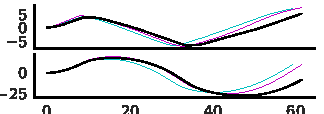
\includegraphics[]{figures/results_optiwise_ID.closed loop zigzag 10_10 stbd.pdf}
        \caption{Zigzag10/10 to starboard.}
        \label{fig:sim_optiwise_10_stbd}
     \end{subfigure}
     \vfill
     \begin{subfigure}[b]{0.40\textwidth}
         \centering
         \includesvg{figures/results_optiwise_ID.closed loop zigzag 20_20 port.svg}
         %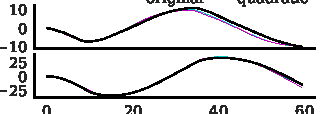
\includegraphics[]{figures/results_optiwise_ID.closed loop zigzag 20_20 port.pdf}
        \caption{Zigzag20/20 to port.}
        \label{fig:sim_optiwise_20_port}
     \end{subfigure}
     \hfill
     \begin{subfigure}[b]{0.40\textwidth}
         \includesvg{figures/results_optiwise_ID.closed loop zigzag 20_20 stbd.svg}
         %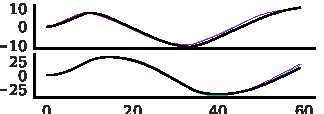
\includegraphics[]{figures/results_optiwise_ID.closed loop zigzag 20_20 stbd.pdf}
        \caption{Zigzag20/20 to starboard.}
        \label{fig:sim_optiwise_20_stbd}
     \end{subfigure}
     
        \caption{Comparison of zigzag tests between Optiwise experiments (black) and simulations with the MMG original (cyan) and MMG quadratic (purple).}
        \label{fig:sim_optiwise}
\end{figure}
\vspace{-1cm}

\begin{figure}[b!]
    \centering
    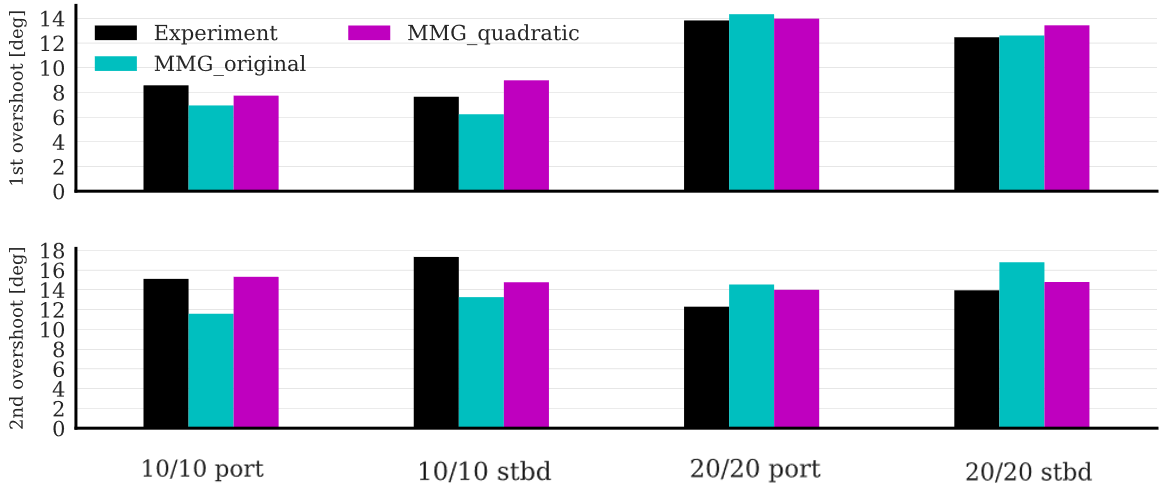
\includegraphics[width=0.9\linewidth, height = 5cm]{figures/results_optiwise_overshoot.png}
    \caption{Overshoot angles from the Optiwise experiments and simulations.}
    \label{fig:overshoots_optiwise}
\end{figure}
\vspace{-0.5cm}
% \begin{figure}[h]
%      \centering
%      \begin{subfigure}[b]{\textwidth}
%          \centering
%          \includesvg{figures/results_optiwise_ID.overshoot1.svg}
%         \caption{First overshoot angles.}
%         \label{fig:overhoots1_optiwise}
%      \end{subfigure}
%      \vfill
%      \begin{subfigure}[b]{\textwidth}
%          \centering
%          \includesvg{figures/results_optiwise_ID.overshoot2.svg}
%         \caption{Second overshoot angles.}
%         \label{fig:overhoots2_optiwise}
%      \end{subfigure}
     
%         \caption{Overshoot angles from the Optiwise experiments and simulations.}
%         \label{fig:overshoots_optiwise}
% \end{figure}